% Options for packages loaded elsewhere
% Options for packages loaded elsewhere
\PassOptionsToPackage{unicode}{hyperref}
\PassOptionsToPackage{hyphens}{url}
\PassOptionsToPackage{dvipsnames,svgnames,x11names}{xcolor}
%
\documentclass[
  english,
  10pt,
  letterpaper,
  DIV=11,
  numbers=noendperiod]{scrartcl}
\usepackage{xcolor}
\usepackage[margin=1in]{geometry}
\usepackage{amsmath,amssymb}
\setcounter{secnumdepth}{5}
\usepackage{iftex}
\ifPDFTeX
  \usepackage[T1]{fontenc}
  \usepackage[utf8]{inputenc}
  \usepackage{textcomp} % provide euro and other symbols
\else % if luatex or xetex
  \usepackage{unicode-math} % this also loads fontspec
  \defaultfontfeatures{Scale=MatchLowercase}
  \defaultfontfeatures[\rmfamily]{Ligatures=TeX,Scale=1}
\fi
\usepackage{lmodern}
\ifPDFTeX\else
  % xetex/luatex font selection
\fi
% Use upquote if available, for straight quotes in verbatim environments
\IfFileExists{upquote.sty}{\usepackage{upquote}}{}
\IfFileExists{microtype.sty}{% use microtype if available
  \usepackage[]{microtype}
  \UseMicrotypeSet[protrusion]{basicmath} % disable protrusion for tt fonts
}{}
\makeatletter
\@ifundefined{KOMAClassName}{% if non-KOMA class
  \IfFileExists{parskip.sty}{%
    \usepackage{parskip}
  }{% else
    \setlength{\parindent}{0pt}
    \setlength{\parskip}{6pt plus 2pt minus 1pt}}
}{% if KOMA class
  \KOMAoptions{parskip=half}}
\makeatother
% Make \paragraph and \subparagraph free-standing
\makeatletter
\ifx\paragraph\undefined\else
  \let\oldparagraph\paragraph
  \renewcommand{\paragraph}{
    \@ifstar
      \xxxParagraphStar
      \xxxParagraphNoStar
  }
  \newcommand{\xxxParagraphStar}[1]{\oldparagraph*{#1}\mbox{}}
  \newcommand{\xxxParagraphNoStar}[1]{\oldparagraph{#1}\mbox{}}
\fi
\ifx\subparagraph\undefined\else
  \let\oldsubparagraph\subparagraph
  \renewcommand{\subparagraph}{
    \@ifstar
      \xxxSubParagraphStar
      \xxxSubParagraphNoStar
  }
  \newcommand{\xxxSubParagraphStar}[1]{\oldsubparagraph*{#1}\mbox{}}
  \newcommand{\xxxSubParagraphNoStar}[1]{\oldsubparagraph{#1}\mbox{}}
\fi
\makeatother


\usepackage{longtable,booktabs,array}
\newcounter{none} % for unnumbered tables
\usepackage{calc} % for calculating minipage widths
% Correct order of tables after \paragraph or \subparagraph
\usepackage{etoolbox}
\makeatletter
\patchcmd\longtable{\par}{\if@noskipsec\mbox{}\fi\par}{}{}
\makeatother
% Allow footnotes in longtable head/foot
\IfFileExists{footnotehyper.sty}{\usepackage{footnotehyper}}{\usepackage{footnote}}
\makesavenoteenv{longtable}
\usepackage{graphicx}
\makeatletter
\newsavebox\pandoc@box
\newcommand*\pandocbounded[1]{% scales image to fit in text height/width
  \sbox\pandoc@box{#1}%
  \Gscale@div\@tempa{\textheight}{\dimexpr\ht\pandoc@box+\dp\pandoc@box\relax}%
  \Gscale@div\@tempb{\linewidth}{\wd\pandoc@box}%
  \ifdim\@tempb\p@<\@tempa\p@\let\@tempa\@tempb\fi% select the smaller of both
  \ifdim\@tempa\p@<\p@\scalebox{\@tempa}{\usebox\pandoc@box}%
  \else\usebox{\pandoc@box}%
  \fi%
}
% Set default figure placement to htbp
\def\fps@figure{htbp}
\makeatother


% definitions for citeproc citations
\NewDocumentCommand\citeproctext{}{}
\NewDocumentCommand\citeproc{mm}{%
  \begingroup\def\citeproctext{#2}\cite{#1}\endgroup}
\makeatletter
 % allow citations to break across lines
 \let\@cite@ofmt\@firstofone
 % avoid brackets around text for \cite:
 \def\@biblabel#1{}
 \def\@cite#1#2{{#1\if@tempswa , #2\fi}}
\makeatother
\newlength{\cslhangindent}
\setlength{\cslhangindent}{1.5em}
\newlength{\csllabelwidth}
\setlength{\csllabelwidth}{3em}
\newenvironment{CSLReferences}[2] % #1 hanging-indent, #2 entry-spacing
 {\begin{list}{}{%
  \setlength{\itemindent}{0pt}
  \setlength{\leftmargin}{0pt}
  \setlength{\parsep}{0pt}
  % turn on hanging indent if param 1 is 1
  \ifodd #1
   \setlength{\leftmargin}{\cslhangindent}
   \setlength{\itemindent}{-1\cslhangindent}
  \fi
  % set entry spacing
  \setlength{\itemsep}{#2\baselineskip}}}
 {\end{list}}
\usepackage{calc}
\newcommand{\CSLBlock}[1]{\hfill\break\parbox[t]{\linewidth}{\strut\ignorespaces#1\strut}}
\newcommand{\CSLLeftMargin}[1]{\parbox[t]{\csllabelwidth}{\strut#1\strut}}
\newcommand{\CSLRightInline}[1]{\parbox[t]{\linewidth - \csllabelwidth}{\strut#1\strut}}
\newcommand{\CSLIndent}[1]{\hspace{\cslhangindent}#1}

\ifLuaTeX
\usepackage[bidi=basic,shorthands=off]{babel}
\else
\usepackage[bidi=default,shorthands=off]{babel}
\fi
\ifLuaTeX
  \usepackage{selnolig} % disable illegal ligatures
\fi


\setlength{\emergencystretch}{3em} % prevent overfull lines

\providecommand{\tightlist}{%
  \setlength{\itemsep}{0pt}\setlength{\parskip}{0pt}}



 


\KOMAoption{captions}{tableheading}
\makeatletter
\@ifpackageloaded{caption}{}{\usepackage{caption}}
\AtBeginDocument{%
\ifdefined\contentsname
  \renewcommand*\contentsname{Table of contents}
\else
  \newcommand\contentsname{Table of contents}
\fi
\ifdefined\listfigurename
  \renewcommand*\listfigurename{List of Figures}
\else
  \newcommand\listfigurename{List of Figures}
\fi
\ifdefined\listtablename
  \renewcommand*\listtablename{List of Tables}
\else
  \newcommand\listtablename{List of Tables}
\fi
\ifdefined\figurename
  \renewcommand*\figurename{Figure}
\else
  \newcommand\figurename{Figure}
\fi
\ifdefined\tablename
  \renewcommand*\tablename{Table}
\else
  \newcommand\tablename{Table}
\fi
}
\@ifpackageloaded{float}{}{\usepackage{float}}
\floatstyle{ruled}
\@ifundefined{c@chapter}{\newfloat{codelisting}{h}{lop}}{\newfloat{codelisting}{h}{lop}[chapter]}
\floatname{codelisting}{Listing}
\newcommand*\listoflistings{\listof{codelisting}{List of Listings}}
\makeatother
\makeatletter
\makeatother
\makeatletter
\@ifpackageloaded{caption}{}{\usepackage{caption}}
\@ifpackageloaded{subcaption}{}{\usepackage{subcaption}}
\makeatother
\usepackage{bookmark}
\IfFileExists{xurl.sty}{\usepackage{xurl}}{} % add URL line breaks if available
\urlstyle{same}
% fallback for those not using the hyperref driver hyperxmp:
\makeatletter
\@ifundefined{xmpquote}{\newcommand{\xmpquote}[1]{#1}}{}
\makeatother
\hypersetup{
  pdftitle={The Economics of De-Peg},
  pdfauthor={Complex--Itô Random-Walk Research Project},
  pdflang={en},
  pdfkeywords={\xmpquote{stablecoins}, \xmpquote{de-peg
risk}, \xmpquote{target zones}, \xmpquote{first
passage}, \xmpquote{reflected Brownian motion}, \xmpquote{hazard
models}},
  colorlinks=true,
  linkcolor={blue},
  filecolor={Maroon},
  citecolor={Blue},
  urlcolor={Blue},
  pdfcreator={LaTeX via pandoc}}


\title{The Economics of De-Peg}
\usepackage{etoolbox}
\makeatletter
\providecommand{\subtitle}[1]{% add subtitle to \maketitle
  \apptocmd{\@title}{\par {\large #1 \par}}{}{}
}
\makeatother
\subtitle{Defended Bands, Credibility Clocks, and Closed-Form De-Peg
Derivatives}
\author{Complex--Itô Random-Walk Research Project}
\date{August 21, 2026}
\begin{document}
\maketitle
\begin{abstract}
Pegged assets --- stablecoins, currency boards, exchange-rate-band
currencies --- trade in a defended band while credible and re-price
discontinuously when credibility fails. We give a two-factor model with
a fully deterministic derivative stack. While the peg is defended, the
log-mispricing is two-sided reflected Brownian motion with the
exponential-trapezoid stationary law \(\pi(y)\propto e^{2by/\sigma^2}\).
De-peg occurs at the first passage of an independent bounded
\emph{credibility factor} \(C_t=X_t/\sqrt{X_t^2+c^2}\) through a
threshold; every law needed by a trading desk is then available in
closed form from the reflection principle --- hitting CDF,
inverse-Gaussian density, perpetual mass --- including the pay-at-hit
transform
\[E[e^{-r\tau}]=\exp\Big((\lambda-\sqrt{\lambda^2+2r/\sigma_z^2})\,
\Delta\Big)\] in which the discount rate enters only as \(r/\sigma_z^2\)
through operational time. Hazard-contingent claims --- shortfall swaps
paying \((K-P_T)^+\) only if the peg broke by \(T\) --- reduce to a
single quadrature over the exact density of \(\tau\) times closed-form
Gaussian components. De-peg probabilities are strongly concave in
horizon (1.7\%, 7.7\%, 17.8\%, 31.7\% at six months through five years
in the reference calibration), capped by the perpetual mass
\(e^{2\lambda\Delta}=48.9\%\) --- a feature any exponential-hazard
specification misses. A perpetual-mass-corrected inverse-transform
simulator validates frequencies within one standard error; we document
the normalization bug that silently doubles hazard frequencies when the
CDF is rescaled instead. No audited framework couples defended bands to
an independent stochastic credibility clock with closed-form contingent
pricing.
\end{abstract}

\renewcommand*\contentsname{Table of contents}
{
\setcounter{tocdepth}{2}
\tableofcontents
}

\textbf{Mathematics Subject Classification (2020):} 91G20, 91B70, 60J60,
60G40.

\textbf{JEL classification:} G13, G15, E42, F31.

\section{Introduction}\label{sec-introduction}

De-peg events are tail events with derivatives written on them:
exchanges list stablecoin de-peg digitals and shortfall-style payouts,
and post-mortems of USDC, Terra, and the 1992 ERM crises document their
severity. The audited literature splits into empirical event studies and
Krugman-type target-zone theory (Krugman 1991); neither prices a book of
de-peg contingent claims under an explicit stochastic credibility
mechanism.

This paper supplies such a mechanism with a fully deterministic pricing
stack, assembled from three exact pieces: defended-band reflection, a
bounded-factor credibility clock, and Gaussian free-float continuation.

\section{Model}\label{sec-model}

\subsection{Defended band}\label{defended-band}

While credible (\(t<\tau\)), the log-mispricing
\(Y_t=\log(P_t/\text{parity})\) is regulated Brownian motion on
\([-\ell,h]\):

\[
dY_t=b\,dt+\sigma\,dW_t+dL_t-dU_t ,
\]

\(L,U\) pushing at the edges. The stationary law is the exponential
trapezoid \(\pi(y)\propto e^{2by/\sigma^2}\) --- uniform at zero drift
(recovered to quadrature precision), tilted toward the intervention edge
otherwise.

\subsection{Credibility clock}\label{credibility-clock}

Independently,

\[
dZ_t=\lambda\sigma_z^2\,dt+\sigma_z\,dW^z_t,\qquad
C_t=f(Z_t)=Z_t/\sqrt{Z_t^2+c^2},\qquad
\tau=\inf\{t:C_t\ge c_*\}.
\]

This is exactly the Milestone-1 bounded-factor first-passage problem:
with \(\Delta=x(c_*)-x(C_0)\) and \(\lambda<0\) (deteriorating
credibility),

\[
P(\tau\le T)=\Phi\!\Big(\frac{\lambda v(T)-\Delta}{\sqrt{v(T)}}\Big)
+e^{2\lambda\Delta}\Phi\!\Big(-\frac{\lambda v(T)+\Delta}{\sqrt{v(T)}}\Big),
\qquad v(T)=\sigma_z^2T,
\]

perpetual mass \(e^{2\lambda\Delta}\), and calendar-time IG density
\(f_\tau(t)=f_u(v(t))\,\sigma_z^2\).

\subsection{Pay-at-hit transform}\label{pay-at-hit-transform}

Since \(\tau_{\text{cal}}=u^*/\sigma_z^2\) with \(u^*\) the
operational-time hitting time of drifted Brownian motion
\((\lambda,B)\),

\[
E[e^{-r\tau};\tau<\infty]
=\exp\Big((\lambda-\sqrt{\lambda^2+2r/\sigma_z^2})\,\Delta\Big):
\]

the raw drift coefficient \(\lambda\) appears directly and the discount
rate enters only scaled --- a compact formula verified against
exact-density quadrature to \(10^{-6}\) after two sign/scale errors were
caught by our own anchors (recorded honestly in Section~\ref{sec-bugs}).

\subsection{Free float and contingent
claims}\label{free-float-and-contingent-claims}

After \(\tau\),
\(\log P_T=y_{\text{exit}}+\mu_f(T-s)+\sigma_f\sqrt{T-s}\,Z\) from the
exit edge. The shortfall swap

\[
V=e^{-rT}\int_0^T f_\tau(s)\;
E\big[(K-e^{y_{\text{exit}}+\mu_f(T-s)+\sigma_f\sqrt{T-s}Z})^+\big]\,ds
\]

prices by ONE quadrature over the exact IG density times Gauss--Hermite
on the Gaussian component --- no simulation anywhere on the pricing
path.

\section{Results}\label{sec-results}

Reference calibration: band \([-2\%,+3\%]\); \(\lambda=-0.25\),
\(\sigma_z=0.9\), \(c=1.1\), \(C_0=0.3\to c_*=0.85\); \(r=5\%\);
\(\mu_f=-15\%\), \(\sigma_f=35\%\).

{\def\LTcaptype{none} % do not increment counter
\begin{longtable}[]{@{}lll@{}}
\toprule\noalign{}
horizon & \(P(\tau\le T)\) & digital \\
\midrule\noalign{}
\endhead
\bottomrule\noalign{}
\endlastfoot
0.5y & 0.01714 & 0.01671 \\
1y & 0.07726 & 0.07349 \\
2y & 0.17785 & 0.16093 \\
5y & 0.31713 & 0.24698 \\
\end{longtable}
}

Concavity is pronounced and perpetual-capped: long-dated digitals can
never exceed \(e^{2\lambda\Delta}=48.9\%\) discounted ---
exponential-hazard specifications, which integrate to one,
systematically overprice them.

Shortfall swaps at \(T=2\) (Figure~\ref{fig-shortfall}):

{\def\LTcaptype{none} % do not increment counter
\begin{longtable}[]{@{}ll@{}}
\toprule\noalign{}
K (\% of parity) & price \\
\midrule\noalign{}
\endhead
\bottomrule\noalign{}
\endlastfoot
70 & 0.004430 \\
80 & 0.008631 \\
90 & 0.014859 \\
95 & 0.018850 \\
98 & 0.021529 \\
\end{longtable}
}

Simulation check: 200k paths, perpetual-mass-corrected inverse-transform
sampling of \(\tau\), projection-reflected band paths, exact free
continuation --- de-peg frequency 0.17800 vs exact 0.17785 (SE 0.00086).

\begin{figure}[tbp]

\centering{

\pandocbounded{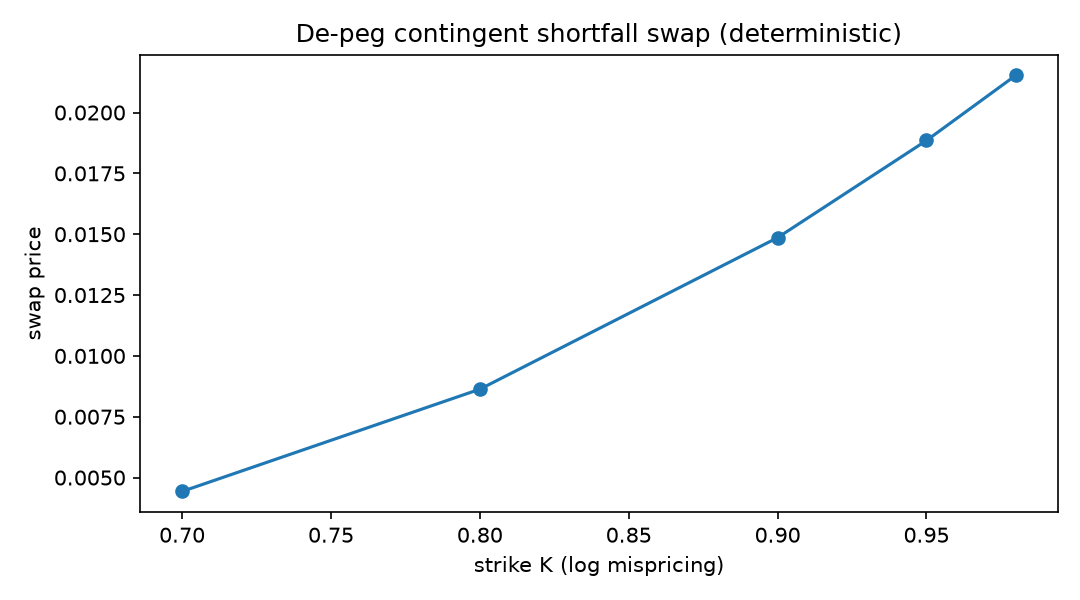
\includegraphics[keepaspectratio]{figures/phase12_shortfall.png}}

}

\caption{\label{fig-shortfall}Shortfall swap prices vs strike
(deterministic).}

\end{figure}%

\section{Two implementation warnings}\label{sec-bugs}

Both were caught by requiring closed forms and simulations to agree:

\begin{enumerate}
\def\labelenumi{\arabic{enumi}.}
\tightlist
\item
  \textbf{Operational-time accounting}: mixing calendar drift
  \(\lambda\sigma_z^2\) with operational-time variance produces wrong
  Laplace transforms; the correct derivation works entirely in
  operational time where the drift is the raw \(\lambda\) and variance
  is unit, then maps discounts through \(r\to r/\sigma_z^2\).
\item
  \textbf{Hazard sampling}: normalizing the truncated hazard CDF to one
  rescales the uniforms and silently multiplies event frequencies by
  \(1/\text{(perpetual mass)}\). Invert the \emph{raw} CDF and mask
  uniforms at the perpetual probability.
\end{enumerate}

\section{Related literature}\label{sec-related}

Target zones (Krugman 1991) value credible bands via smooth pasting but
carry no stochastic credibility hazard and no contingent stack;
speculative- attack models are qualitative about timing; stablecoin
de-peg studies are empirical. First-passage Laplace transforms and
reflected Brownian stationary laws are classical tools we assemble, not
contributions; the contribution is the two-factor coupling with its
deterministic derivative stack and the falsifiable concavity prediction.

\section{Conclusion}\label{sec-conclusion}

A peg is a derivative on its own credibility. Once credibility is
modeled as a bounded factor, every de-peg instrument prices in closed
form or a single quadrature --- and the resulting term structures carry
a testable signature (perpetual-mass concavity) that distinguishes the
mechanism from memoryless hazards.

\section{Reproducibility}\label{sec-repro}

Environment: conda \texttt{phase3-paper} (Python 3.12.13, numpy 2.5.1,
scipy 1.18.0). Notebook \texttt{notebooks/phase12\_peg.ipynb}
(\textasciitilde3 s, seed 20260821); module \texttt{phase12\_peg.py};
tests \texttt{tests/test\_phase12\_peg.py} (7/7).

\protect\phantomsection\label{refs}
\begin{CSLReferences}{1}{1}
\bibitem[\citeproctext]{ref-krugman1991}
Krugman, Paul. 1991. \emph{Target Zones and Exchange Rate Dynamics}.

\end{CSLReferences}




\end{document}
